% !TeX spellcheck = de_DE
\documentclass[10pt,a4paper]{article}
\usepackage[latin1]{inputenc}
\usepackage{amsmath}
\usepackage{amsfonts}
\usepackage{amssymb}
\usepackage{graphicx}
\usepackage{hyperref}
\usepackage[paperheight=21cm,left=1cm,right=1cm]{geometry}
\pagestyle{empty}
\setlength\parindent{0pt}

\begin{document}

\section{Den playground auschecken}

Rechtsklick in den leeren Bereich, dann \emph{SVN Checkout...}

\begin{center}
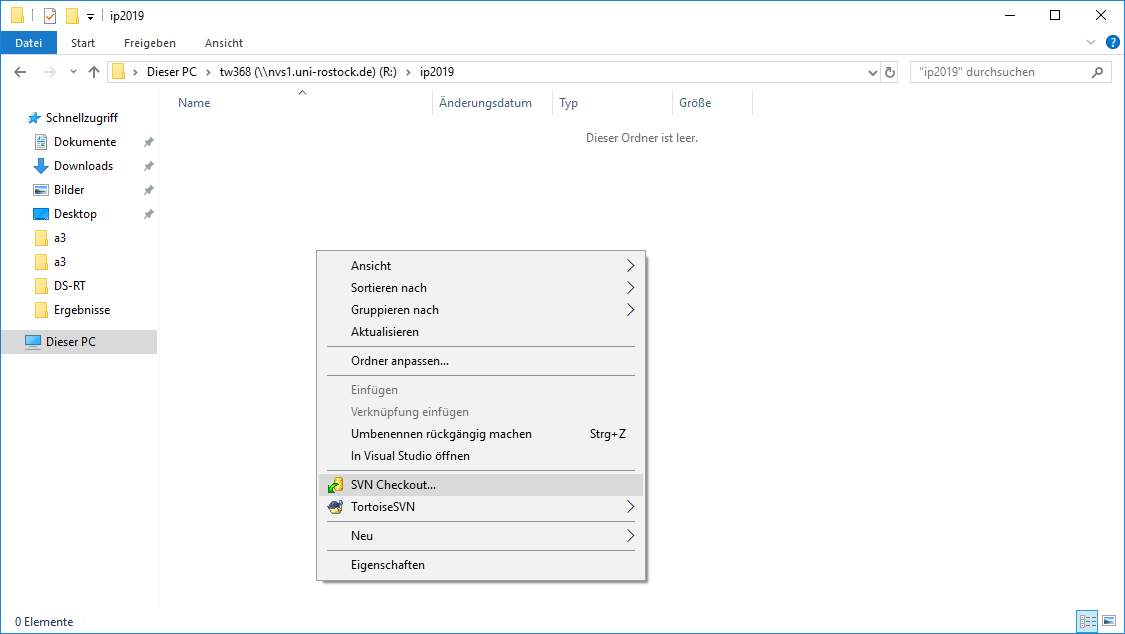
\includegraphics[width=\linewidth]{t1}
\end{center}

\clearpage

URL zum playground im Repository (\url{https://svn.informatik.uni-rostock.de/lehre/ip2019/playground/}) und Pfad f�r lokale Arbeitskopie (auf Laufwerk \texttt{R:}) eintragen.
Ggf.\ mit ITMZ Account authentifizieren.

\begin{center}
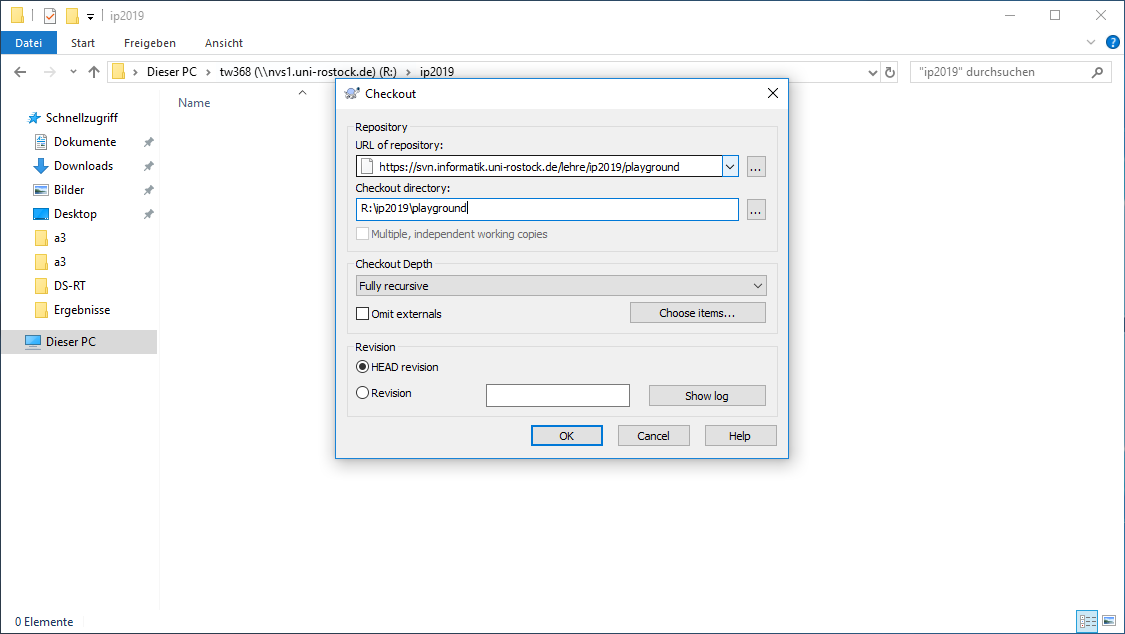
\includegraphics[width=\linewidth]{t2}
\end{center}

\clearpage

Checkout beobachten, dann Fenster mit \emph{OK} schlie�en.

\begin{center}
	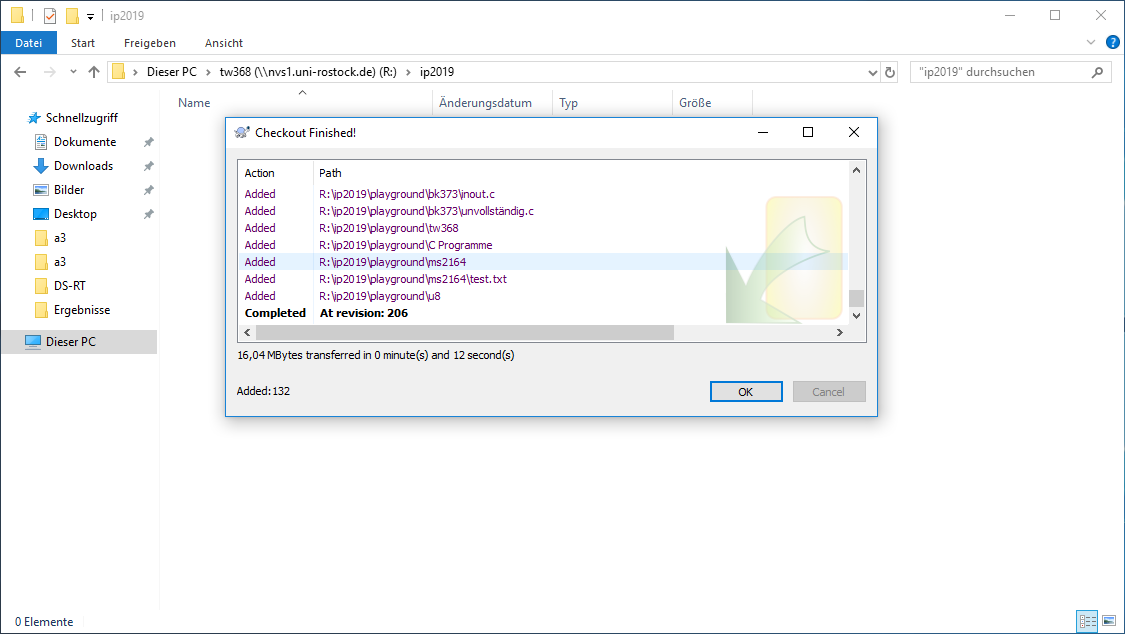
\includegraphics[width=\linewidth]{t3}
\end{center}

\clearpage

Fertig!

\begin{center}
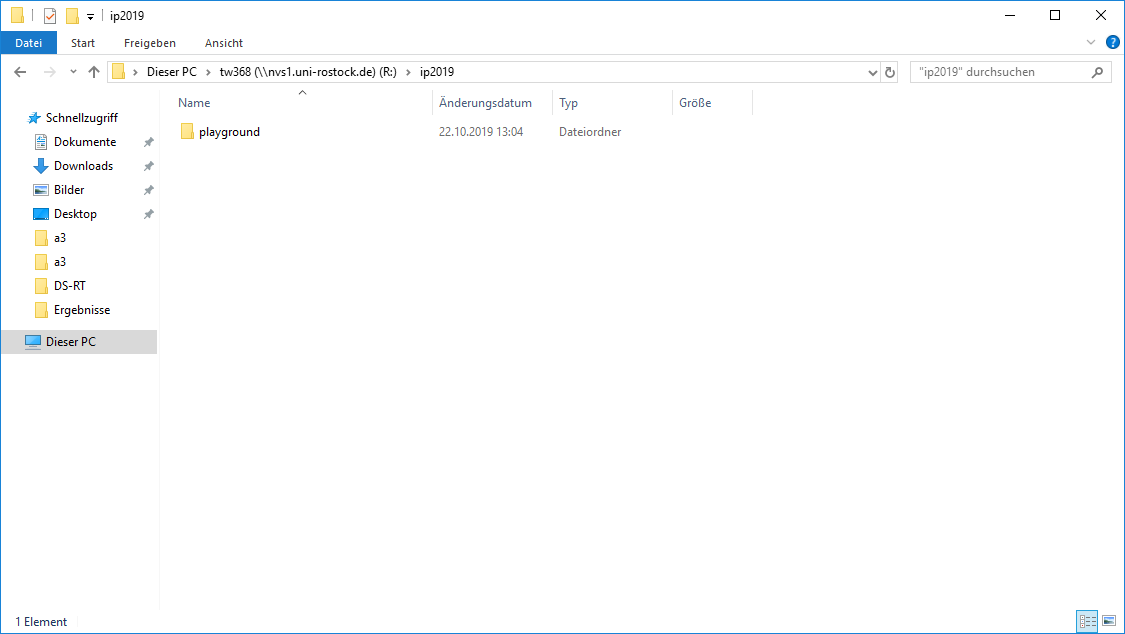
\includegraphics[width=\linewidth]{t4}
\end{center}

\clearpage


\section{Einen Ordner commiten}

Wir k�nnen im ausgecheckten Ordner einen Ordner anlegen.

\begin{center}
	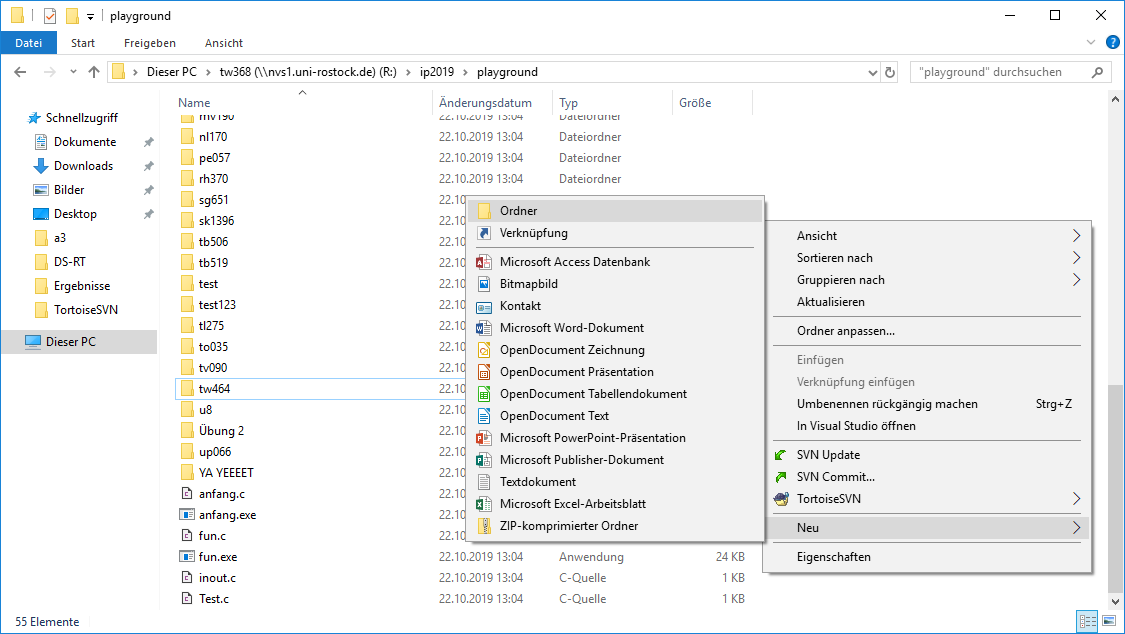
\includegraphics[width=\linewidth]{t5}
\end{center}

\clearpage

\begin{center}
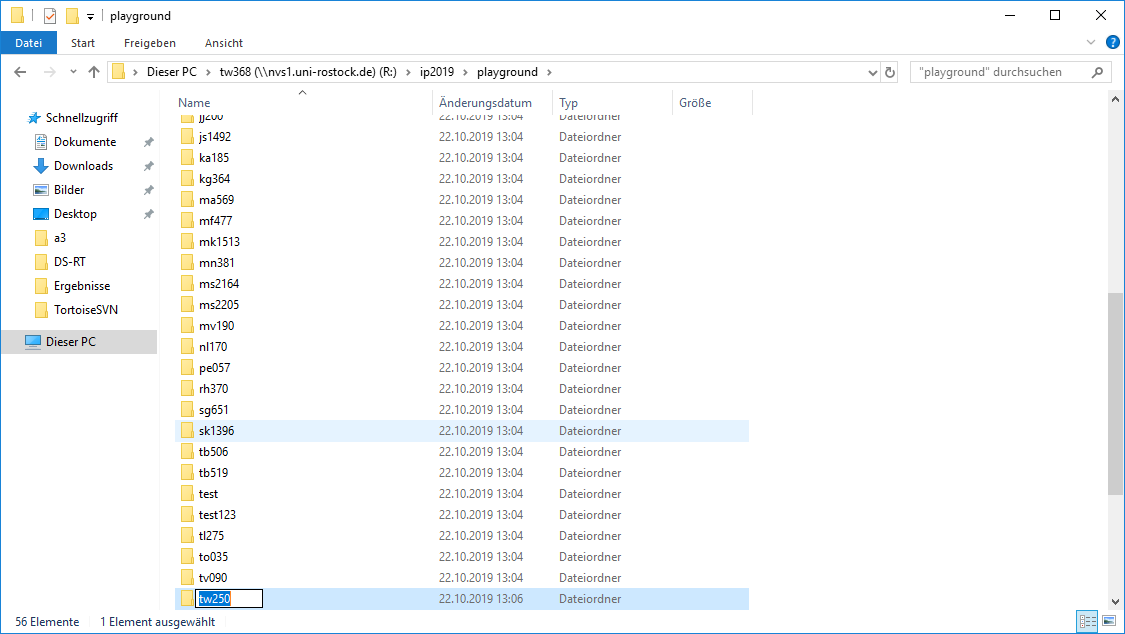
\includegraphics[width=\linewidth]{t6}
\end{center}

\clearpage

Wir f�gen ihn dem Repository hinzu (\emph{Add...}) und stellen ihn damit unter Versionsverwaltung.

\begin{center}
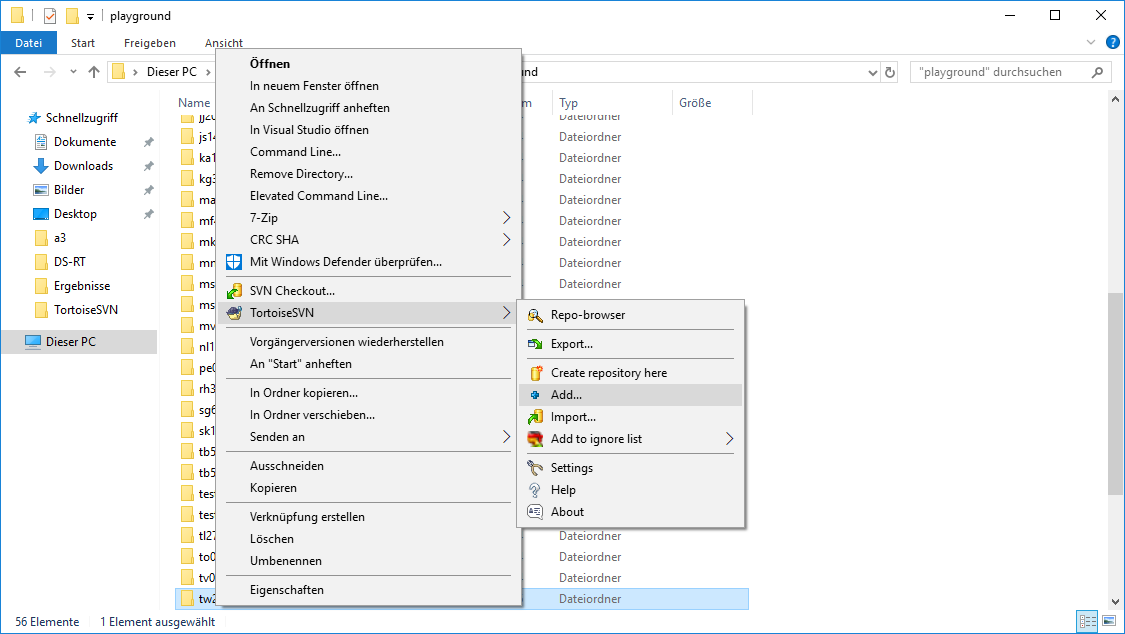
\includegraphics[width=\linewidth]{t7}
\end{center}

\clearpage

Hinzuzuf�gende Ordner und Dateien anticken und dann \emph{OK}.

\begin{center}
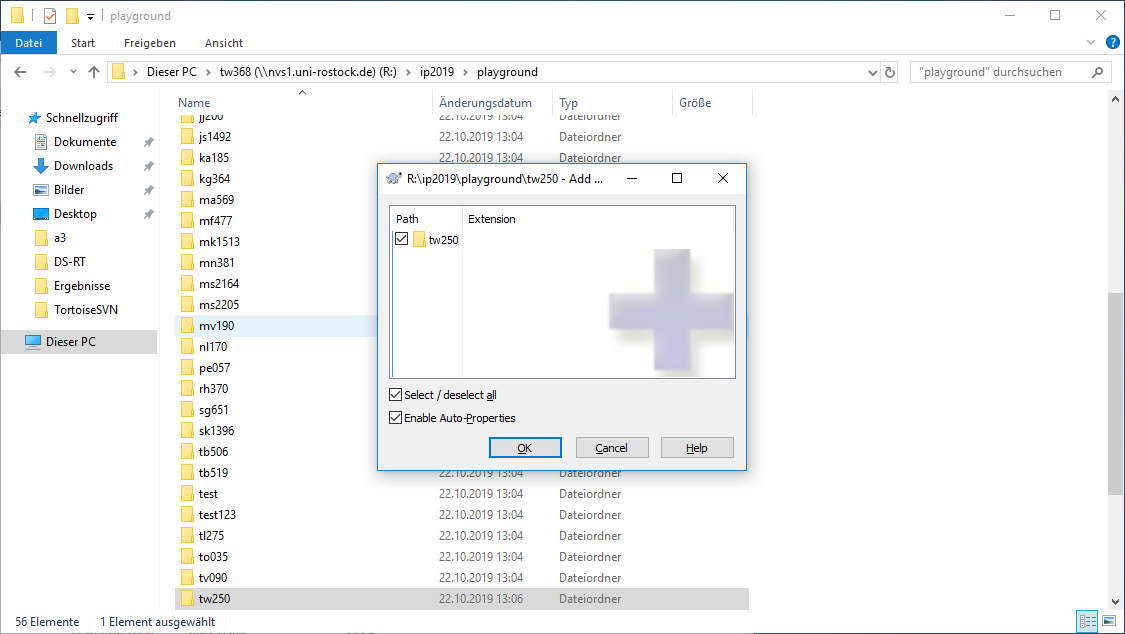
\includegraphics[width=\linewidth]{t8}
\end{center}

\clearpage


\emph{OK}.

\begin{center}
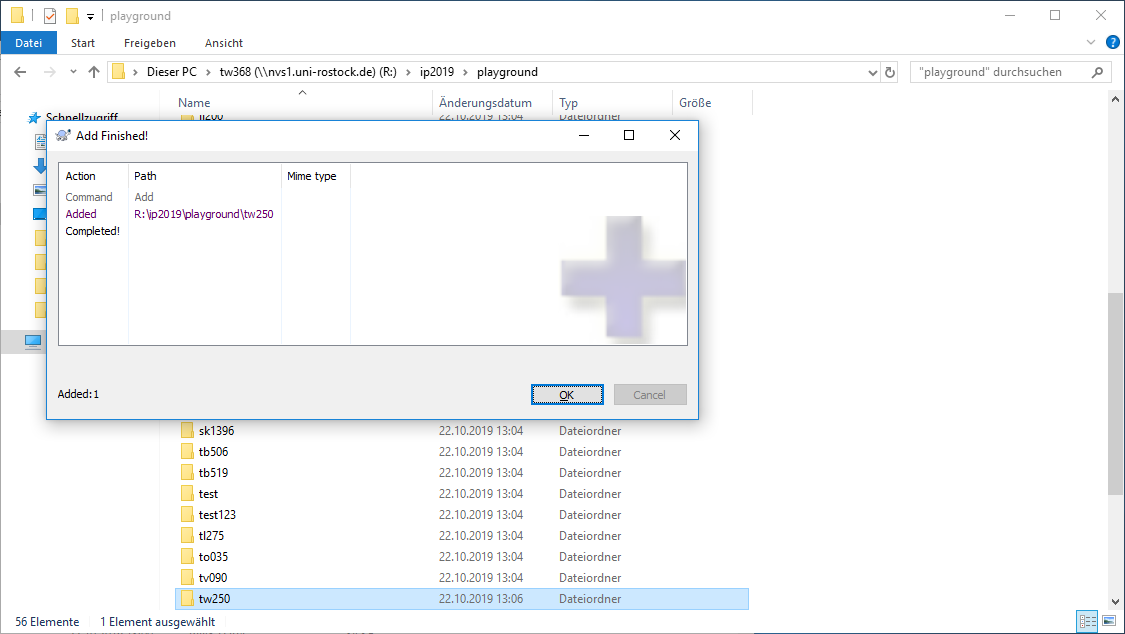
\includegraphics[width=\linewidth]{t9}
\end{center}

\clearpage

Nun k�nnen wir den hinzugef�gten Ordner commiten.

\begin{center}
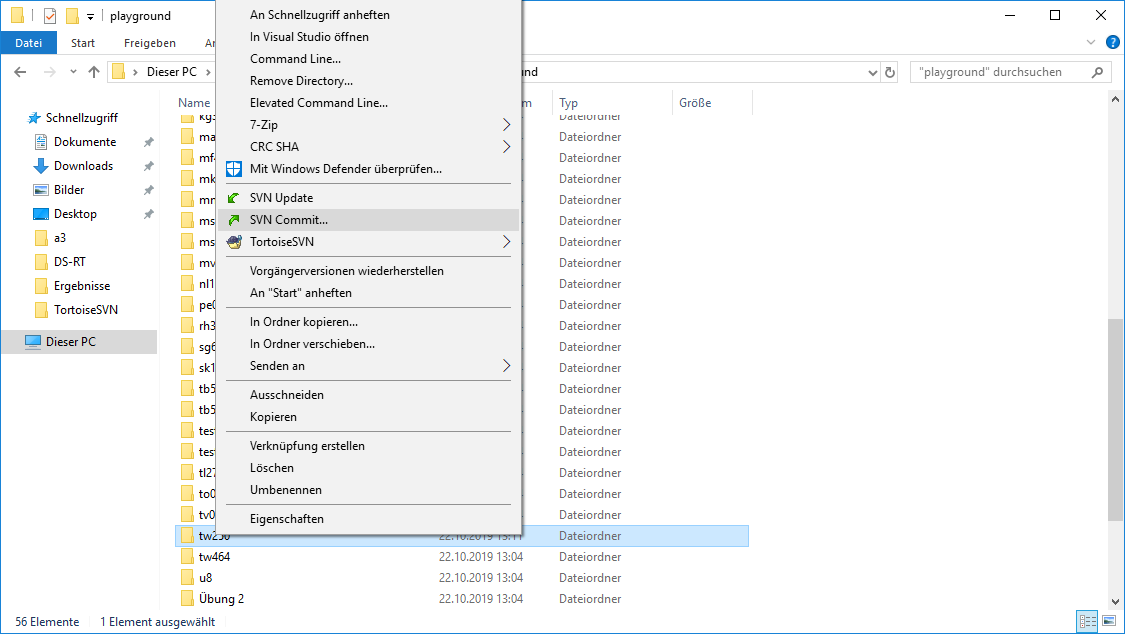
\includegraphics[width=\linewidth]{t10}
\end{center}

\clearpage

Dazu m�ssen wir einen Text eingeben, der unsere �nderungen beschreibt.

\begin{center}
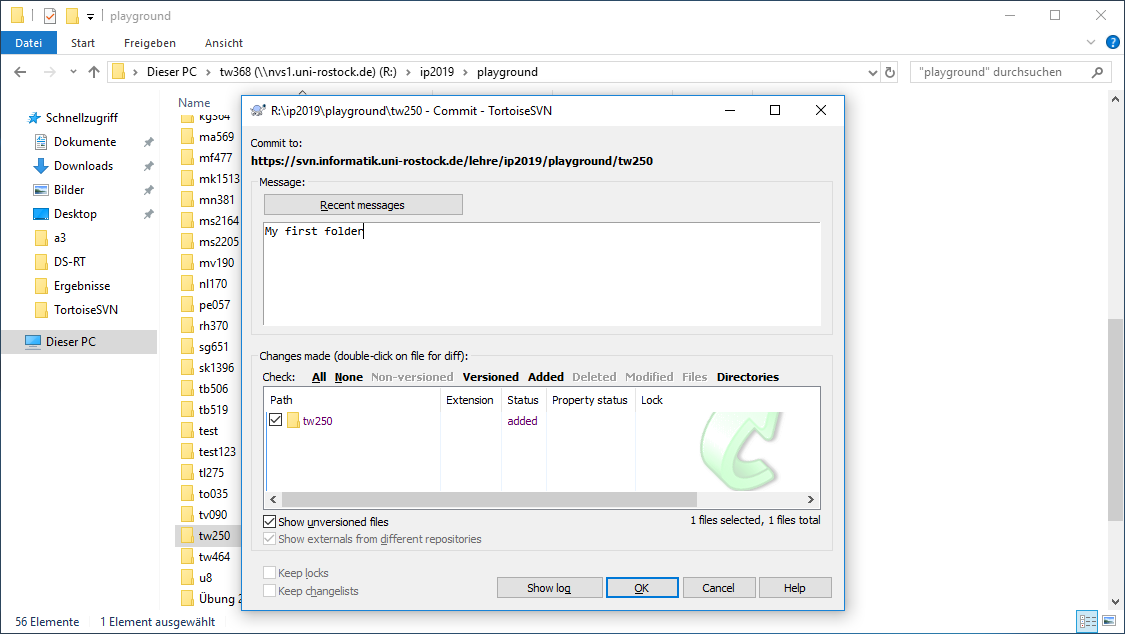
\includegraphics[width=\linewidth]{t11}
\end{center}

\clearpage

Fertig.

\begin{center}
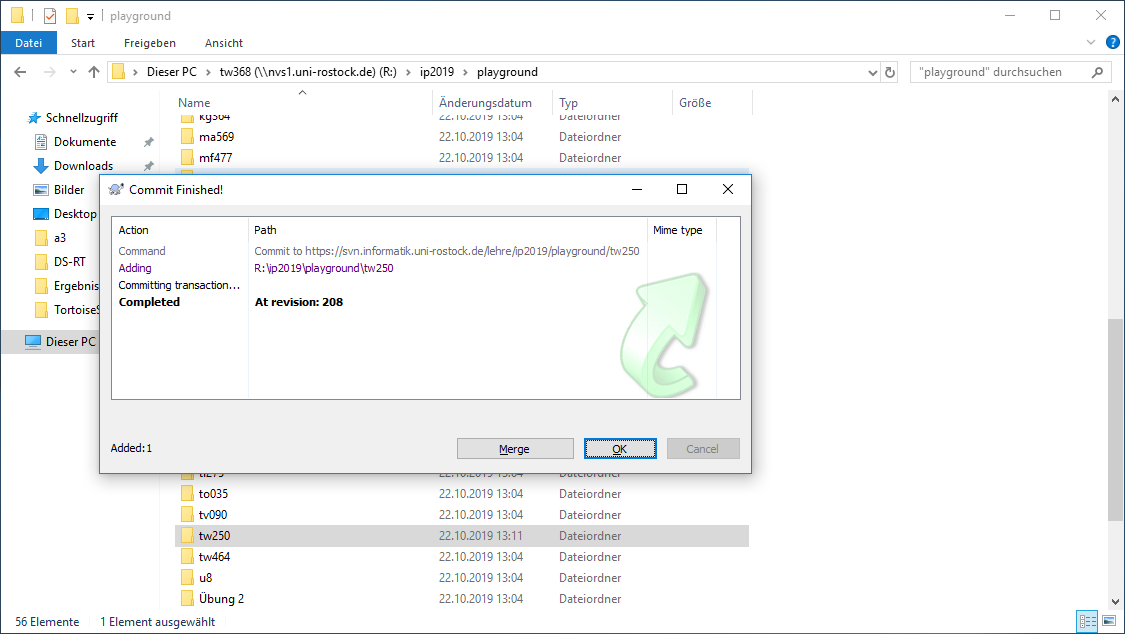
\includegraphics[width=\linewidth]{t12}
\end{center}

\clearpage

\section{Eine Datei commiten}

Wir k�nnen in unserem Ordner eine Datei erstellen.

\begin{center}
	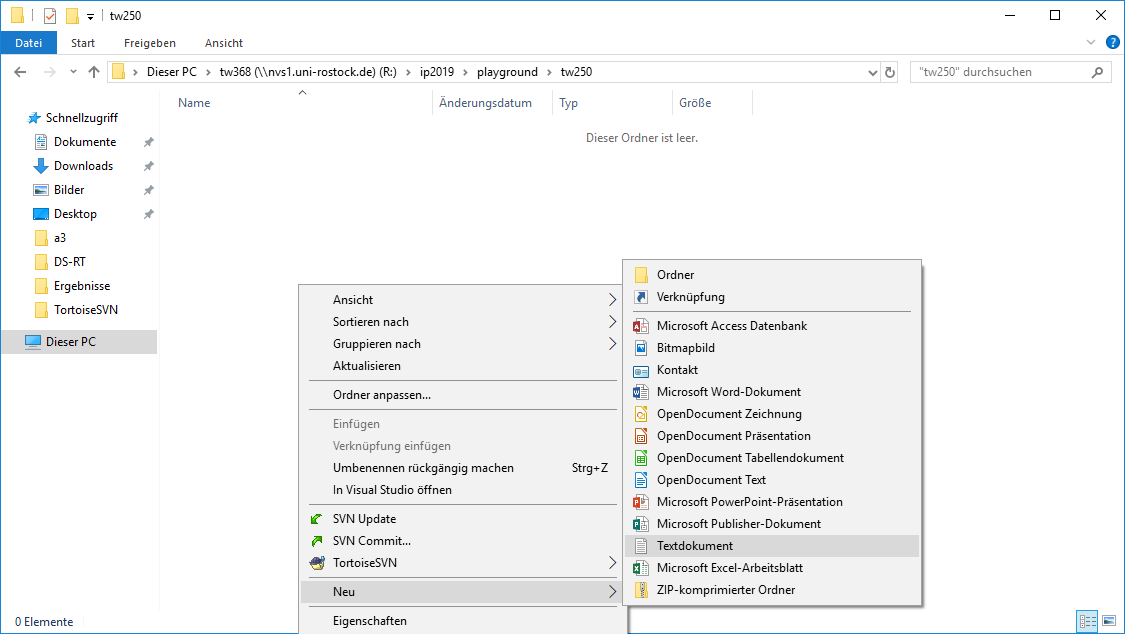
\includegraphics[width=\linewidth]{t13}
\end{center}

\clearpage

Wir erstellen eine C-Quellcodedatei.

\begin{center}
	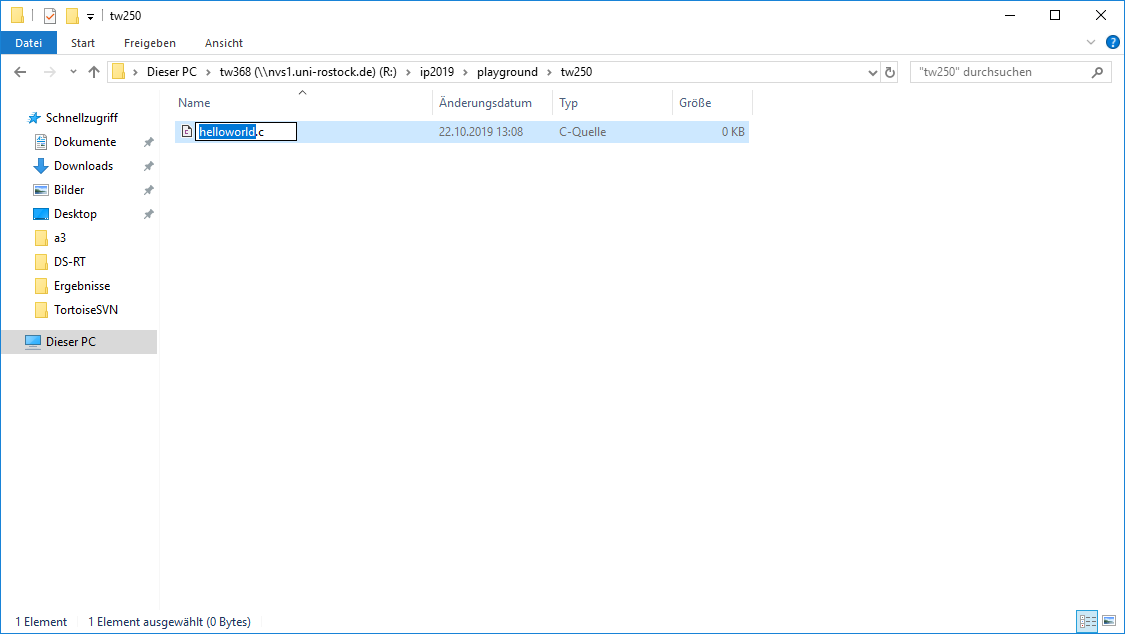
\includegraphics[width=\linewidth]{t14}
\end{center}

\clearpage

Um die Datei zu commiten, gehen wir vor wie bei einem Ordner. Erst die neue Datei hinzuf�gen...

\begin{center}
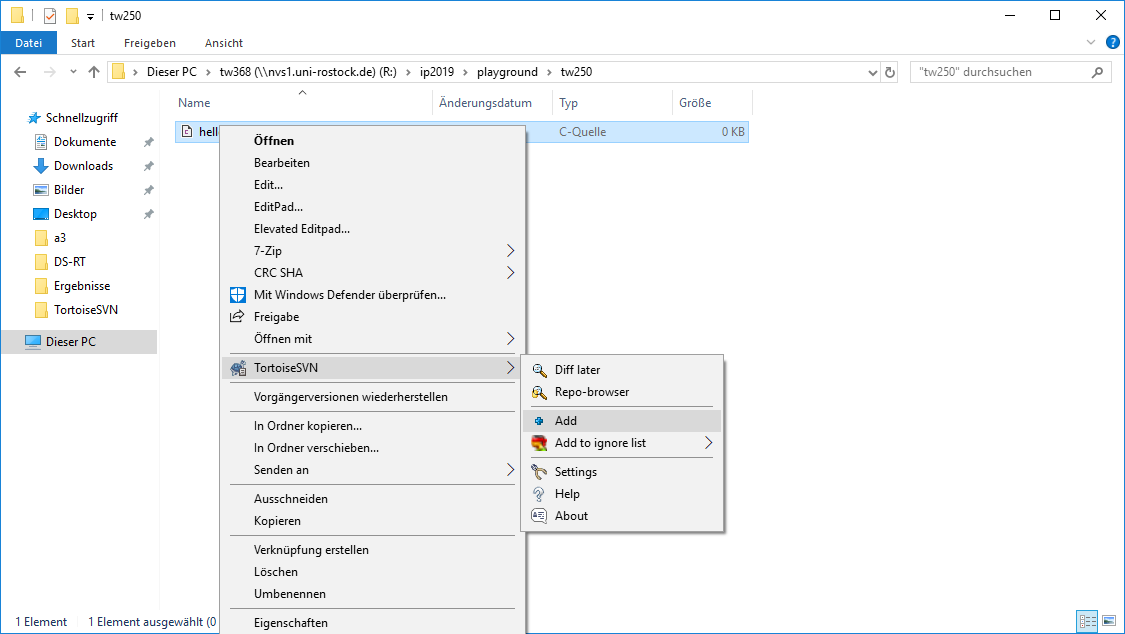
\includegraphics[width=\linewidth]{t15}
\end{center}

\clearpage

...dann commiten...

\begin{center}
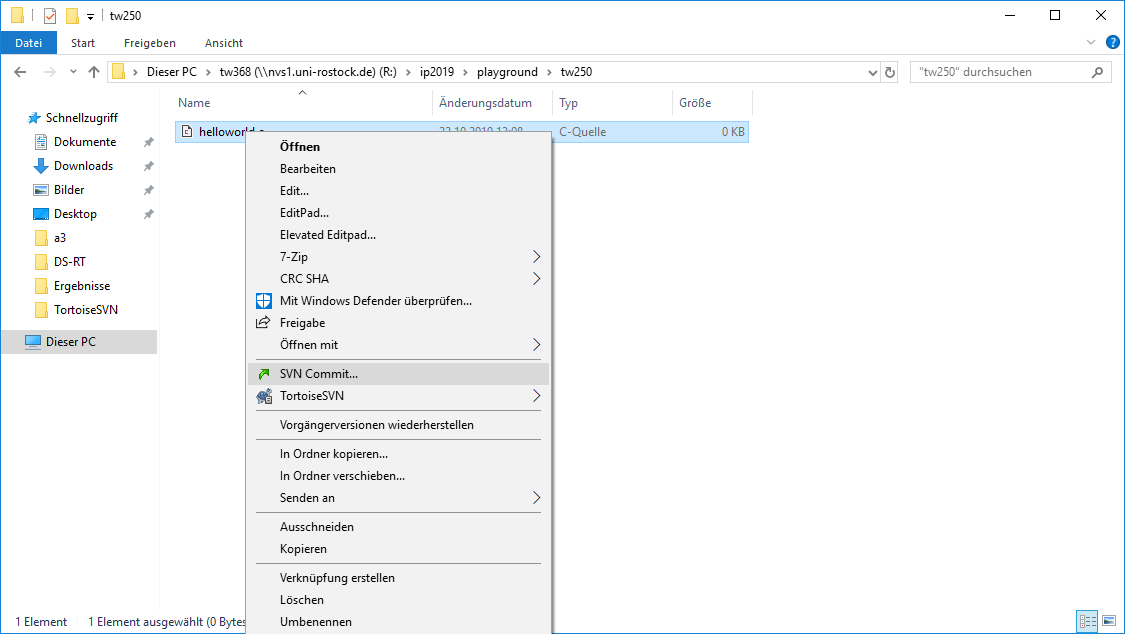
\includegraphics[width=\linewidth]{t16}
\end{center}

\clearpage

...und dazu eine passende Commit Message angeben

\begin{center}
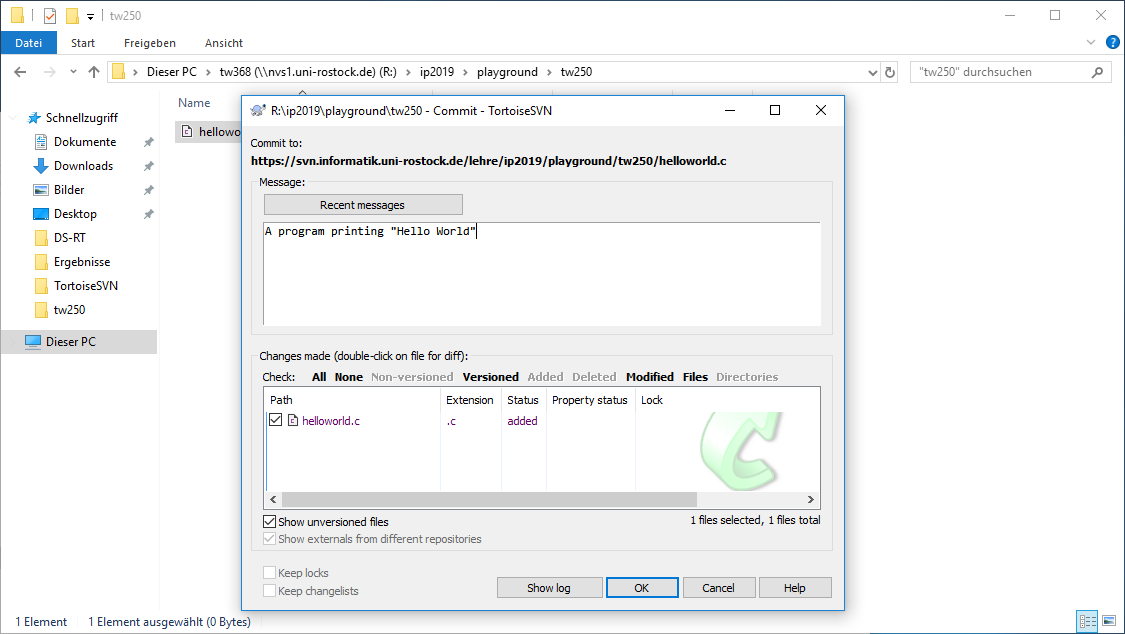
\includegraphics[width=\linewidth]{t17}
\end{center}

\clearpage

Fertig!

\begin{center}
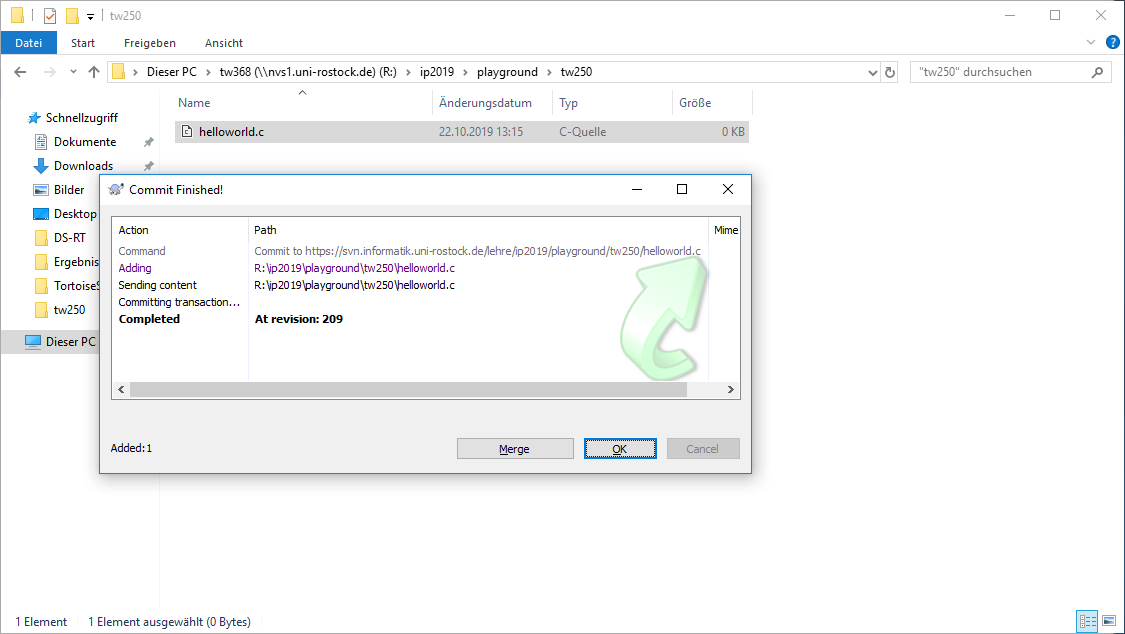
\includegraphics[width=\linewidth]{t18}
\end{center}

\clearpage

\section{�nderungen commiten}

Wenn der Inhalt einer Datei unter Versionsverwaltung ge�ndert wurde, kann sie erneut commitet werden.

\begin{center}
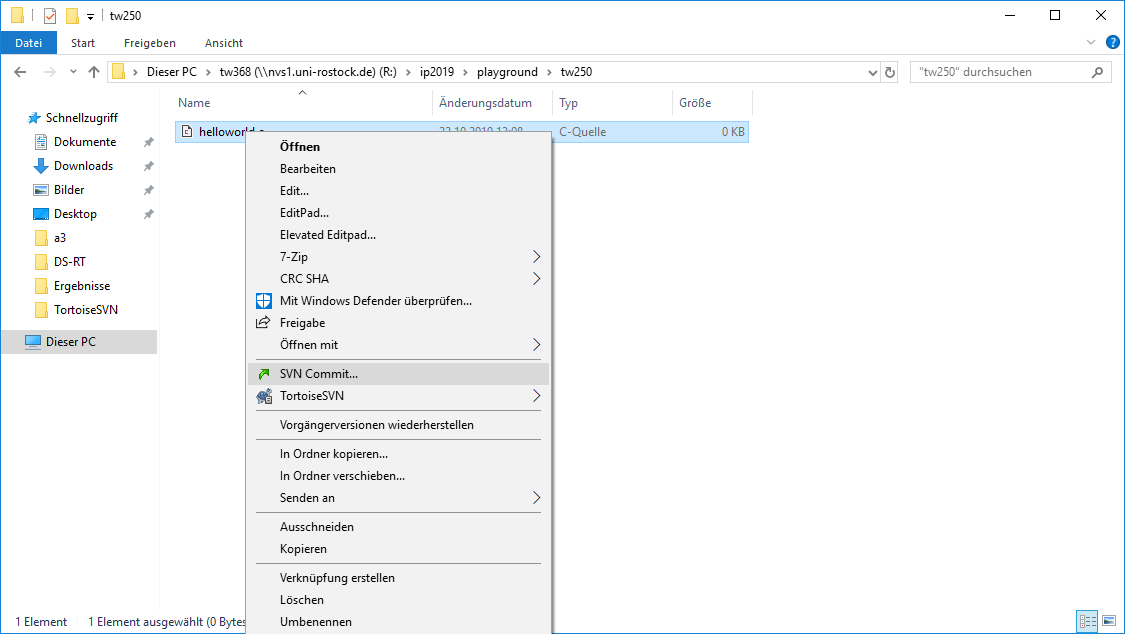
\includegraphics[width=\linewidth]{t16}
\end{center}

\clearpage

Wir m�ssen dazu wieder eine passende Commit Message angeben.

\begin{center}
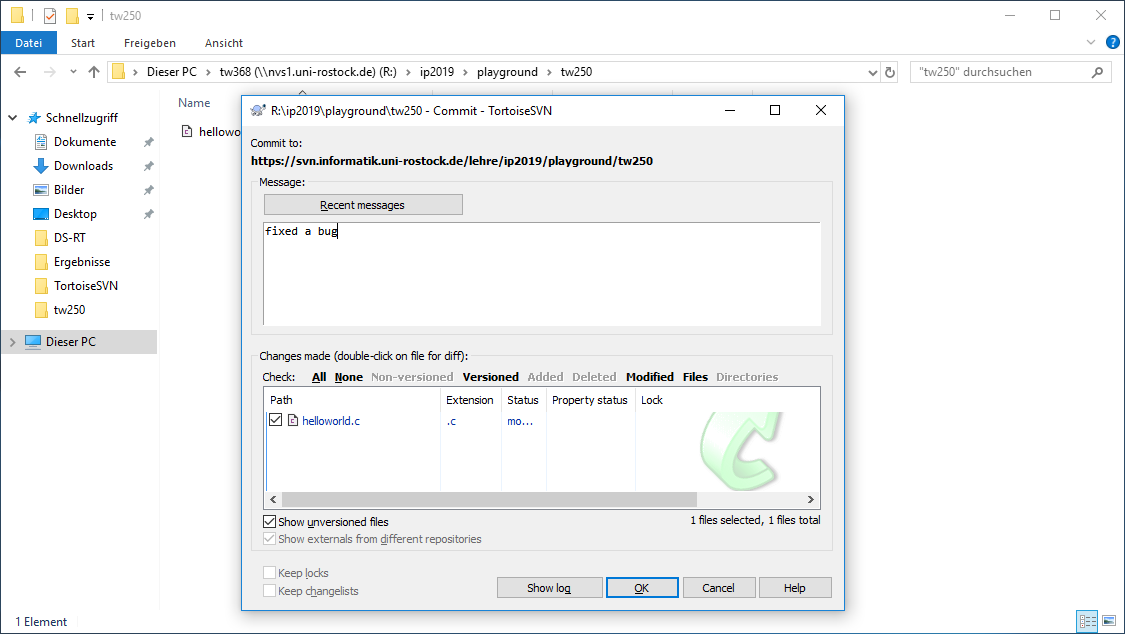
\includegraphics[width=\linewidth]{t21}
\end{center}

\clearpage

Fertig!

\begin{center}
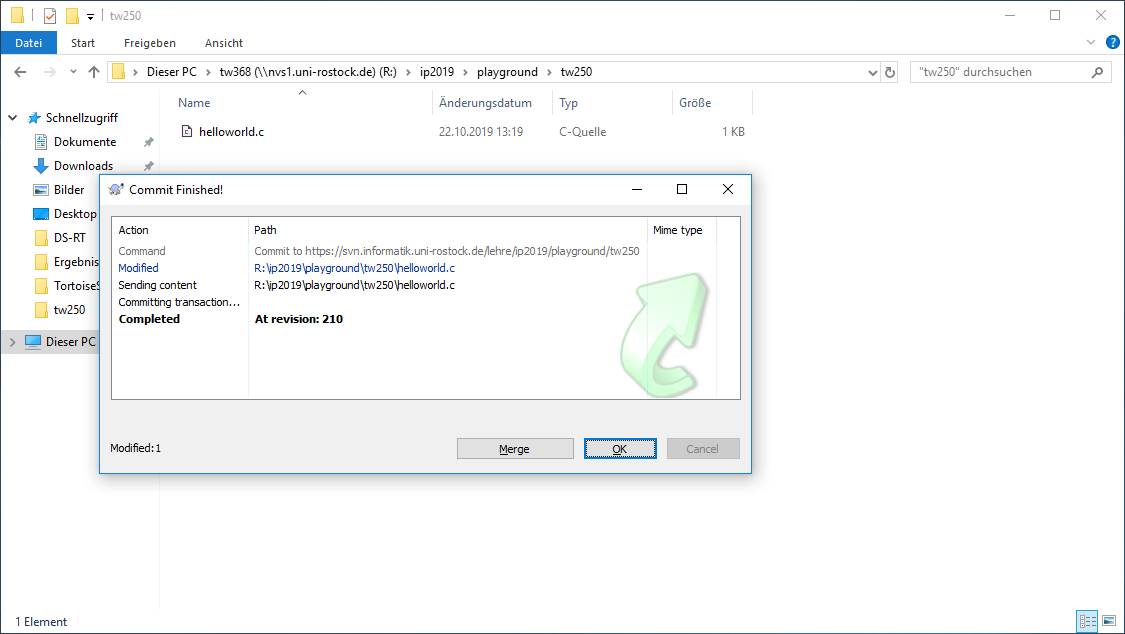
\includegraphics[width=\linewidth]{t22}
\end{center}

\clearpage

\section{Verlauf ansehen}

In dem Verlauf kann man alle Versionen der Datei sehen, die commitet wurden.

\begin{center}
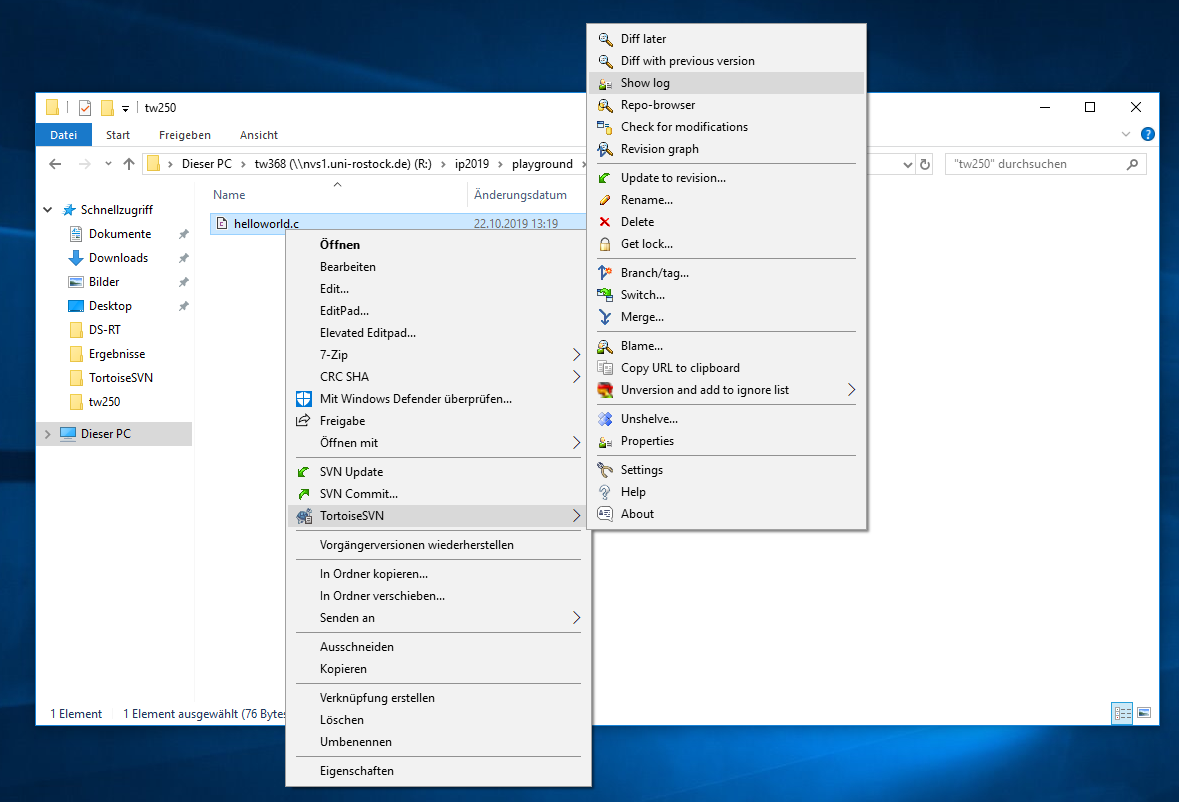
\includegraphics[width=\linewidth]{t23}
\end{center}

\clearpage

\begin{center}
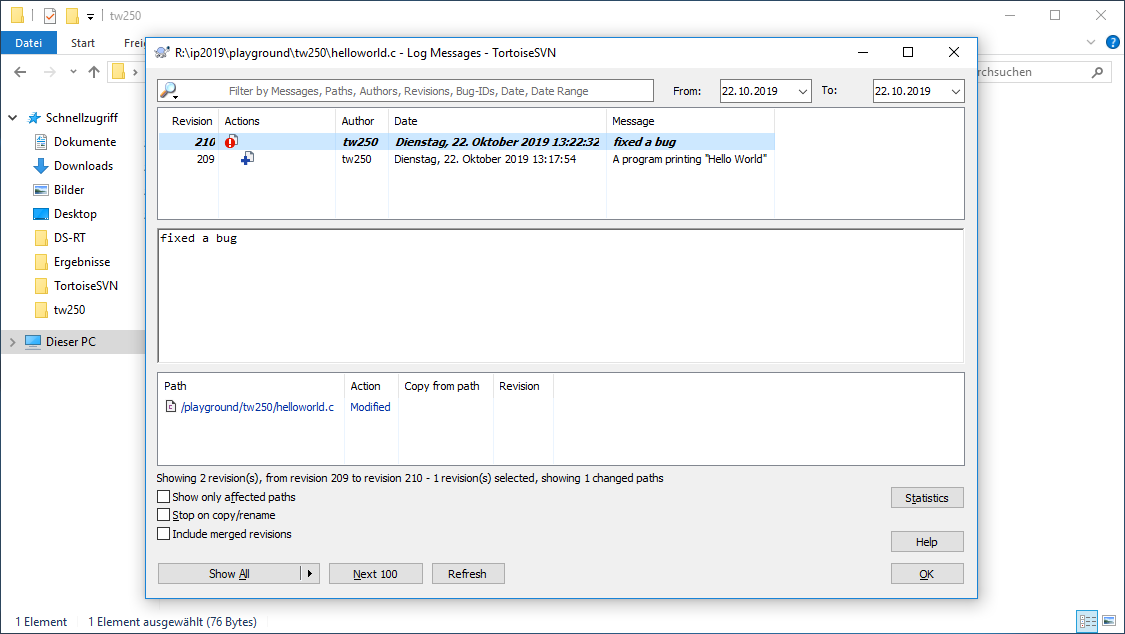
\includegraphics[width=\linewidth]{t24}
\end{center}

\clearpage

\section{Auf aktuellen Stand updaten}

Per Update kann man den aktuellen Stand vom Server holen.
Um den ganzen Ordner zu updaten, in den wei�en Bereich rechtsklicken.

\begin{center}
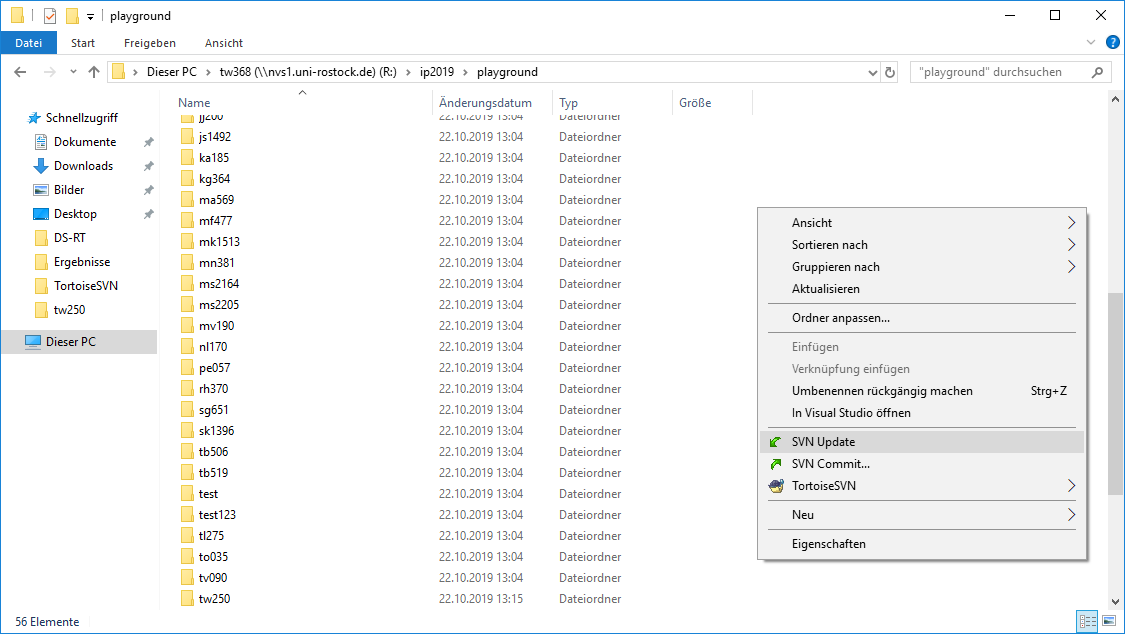
\includegraphics[width=\linewidth]{t19}
\end{center}

\clearpage

Fertig!

\begin{center}
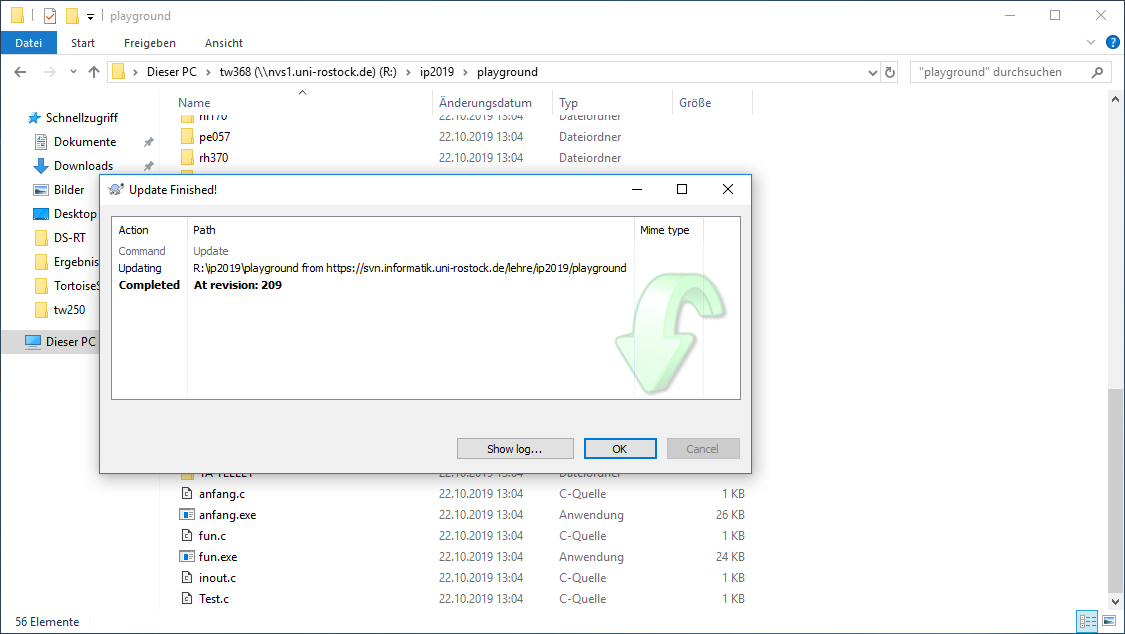
\includegraphics[width=\linewidth]{t20}
\end{center}


\end{document}